%% Преамбула TeX-файла

% 1. Стиль и язык
\documentclass[utf8x]{G7-32} % Стиль (по умолчанию будет 14pt)
\usepackage[T2A]{fontenc}
\usepackage[russian]{babel}
\setcounter{page}{4}
% Остальные стандартные настройки убраны в preamble.inc.tex.
%%==========================================%%
%% Для избежания переносов слов
\usepackage{ragged2e}
\usepackage{microtype}

\justifying
\sloppy
\tolerance=500
\hyphenpenalty=10000
\emergencystretch=3em
%%==========================================%%

% Настройки стиля ГОСТ 7-32
% Для начала определяем, хотим мы или нет, чтобы рисунки и таблицы нумеровались в пределах раздела, или нам нужна сквозная нумерация.
\EqInChapter % формулы будут нумероваться в пределах раздела
\TableInChapter % таблицы будут нумероваться в пределах раздела
\PicInChapter % рисунки будут нумероваться в пределах раздела

% Добавляем гипертекстовое оглавление в PDF
\usepackage[
bookmarks=true, colorlinks=true, unicode=true,
urlcolor=black,linkcolor=black, anchorcolor=black,
citecolor=black, menucolor=black, filecolor=black,
]{hyperref}

%Величина «красной строки»


\usepackage[tableposition=top,singlelinecheck=false]{caption}
%\usepackage{subcaption}

\DeclareCaptionLabelFormat{gostfigure}{Рисунок #2}
\DeclareCaptionLabelFormat{gosttable}{Таблица #2}
\DeclareCaptionLabelSeparator{gost}{~---~}
% Можно разбивать длинные таблицы вручную, оформляя каждую как table. В этом случае для продолжений таблицы нужно создать отдельный стиль заголовка
\DeclareCaptionLabelFormat{continued}{Продолжение таблицы~#2}
\captionsetup*[ContinuedFloat]{labelformat=continued}
\captionsetup{labelsep=gost}
\captionsetup*[figure]{labelformat=gostfigure, justification=centering,font={small, bf}}  % выравнивание по центру
\captionsetup*[table]{hangindent=-10pt, indention=0pt,parindent=0pt,margin=0pt,labelformat=gosttable,justification=raggedright,font={small,it}}
\captionsetup*[lstlisting]{font={small, it}}

% Изменение начертания шрифта --- после чего выглядит таймсоподобно.
% apt-get install scalable-cyrfonts-tex

\IfFileExists{cyrtimes.sty}
    {
        \usepackage{cyrtimespatched}
    }
    {
        % А если Times нету, то будет CM...
    }

\usepackage{graphicx}   % Пакет для включения рисунков
%расположение графики
\graphicspath{{images/}{figures/}{screnshots/}{../images/}}  % папки с картинками

% С такими оно полями оно работает по-умолчанию:
% \RequirePackage[left=20mm,right=10mm,top=20mm,bottom=20mm,headsep=0pt]{geometry}
% Если вас тошнит от поля в 10мм --- увеличивайте до 20-ти, ну и про переплёт не забывайте:
\geometry{right=10mm}
\geometry{left=30mm}


% Пакет Tikz
\usepackage{tikz}
\usetikzlibrary{arrows,positioning,shadows}

% Произвольная нумерация списков.
\usepackage{enumerate}

% ячейки в несколько строчек
\usepackage{multirow}

% itemize внутри tabular
\usepackage{paralist,array}


% Настройки листингов.
% 8 Листинги

\usepackage{listings}

% Значения по умолчанию
\lstset{
  basicstyle= \footnotesize\ttfamily,
  breakatwhitespace=true,% разрыв строк только на whitespacce
  breaklines=true,       % переносить длинные строки
%   captionpos=b,          % подписи снизу -- вроде не надо
  inputencoding=koi8-r,
  numbers=left,          % нумерация слева
  numberstyle=\footnotesize,
  showspaces=false,      % показывать пробелы подчеркиваниями -- идиотизм 70-х годов
  showstringspaces=false,
  showtabs=false,        % и табы тоже
  stepnumber=1,
  tabsize=4,              % кому нужны табы по 8 символов?
  frame=single
}

% Стиль для псевдокода: строчки обычно короткие, поэтому размер шрифта побольше
\lstdefinestyle{pseudocode}{
  basicstyle=\small\ttfamily,
  keywordstyle=\color{black}\bfseries\underbar,
  language=Pseudocode,
  numberstyle=\footnotesize,
  commentstyle=\footnotesize\it\texttt
}

% Стиль для обычного кода: маленький шрифт
\lstdefinestyle{realcode}{
  basicstyle=\scriptsize,
  numberstyle=\footnotesize
}

% Стиль для коротких кусков обычного кода: средний шрифт
\lstdefinestyle{simplecode}{
  basicstyle=\footnotesize,
  numberstyle=\footnotesize
}

% Стиль для BNF
\lstdefinestyle{grammar}{
  basicstyle=\footnotesize,
  numberstyle=\footnotesize,
  stringstyle=\bfseries\ttfamily,
  language=BNF
}

% Определим свой язык для написания псевдокодов на основе Python
\lstdefinelanguage[]{Pseudocode}[]{Python}{
  morekeywords={each,empty,wait,do},% ключевые слова добавлять сюда
  morecomment=[s]{\{}{\}},% комменты {а-ля Pascal} смотрятся нагляднее
  literate=% а сюда добавлять операторы, которые хотите отображать как мат. символы
    {->}{\ensuremath{$\rightarrow$}~}2%
    {<-}{\ensuremath{$\leftarrow$}~}2%
    {:=}{\ensuremath{$\leftarrow$}~}2%
    {<--}{\ensuremath{$\Longleftarrow$}~}2%
}[keywords,comments]

% Свой язык для задания грамматик в BNF
\lstdefinelanguage[]{BNF}[]{}{
  morekeywords={},
  morecomment=[s]{@}{@},
  morestring=[b]",%
  literate=%
    {->}{\ensuremath{$\rightarrow$}~}2%
    {*}{\ensuremath{$^*$}~}2%
    {+}{\ensuremath{$^+$}~}2%
    {|}{\ensuremath{$|$}~}2%
}[keywords,comments,strings]

% Подписи к листингам на русском языке.
\renewcommand\lstlistingname{\cyr\CYRL\cyri\cyrs\cyrt\cyri\cyrn\cyrg}
\renewcommand\lstlistlistingname{\cyr\CYRL\cyri\cyrs\cyrt\cyri\cyrn\cyrg\cyri}


% Полезные макросы листингов.
% Любимые команды
\newcommand{\Code}[1]{\textbf{#1}}


\renewcommand{\rmdefault}{ftm}

\begin{document}


 % выключает нумерацию ВСЕГО; здесь начинаются ненумерованные главы: реферат, введение, глоссарий, сокращения и прочее.

% Команды \breakingbeforechapters и \nonbreakingbeforechapters
% управляют разрывом страницы перед главами.
% По-умолчанию страница разрывается.

% \nobreakingbeforechapters
% \breakingbeforechapters

%% Также можно использовать \Referat, как в оригинале
\begin{abstract}
Это пример каркаса расчётно-пояснительной записки, желательный к использованию в РПЗ проекта по курсу РСОИ.

Данный опус, как и более новые версии этого документа, можно взять по адресу (\url{https://github.com/rominf/latex-g7-32}).

Текст в документе носит совершенно абстрактный характер.
\end{abstract}

%%% Local Variables: 
%%% mode: latex
%%% TeX-master: "rpz"
%%% End: 

% Также можно использовать \Referat, как в оригинале
\begin{abstract}
	

	\newcounter{totfigures}
	\newcounter{tottables}
	\makeatletter
	\AtEndDocument{%
		\addtocounter{totfigures}{\value{figure}}%
		\addtocounter{tottables}{\value{table}}%
		\immediate\write\@mainaux{%
			\string\gdef\string\totfig{\number\value{totfigures}}%
			\string\gdef\string\tottab{\number\value{tottables}}%    
		}%
	}
	\makeatother
	
	
	\pretocmd{\chapter}{\addtocounter{totfigures}{\value{figure}}}{}{}
	\pretocmd{\chapter}{\addtocounter{tottables}{\value{table}}}{}{}
	% ...
	Дипломная работа: \pageref*{LastPage}~с., \totfig~рис., \tottab~табл...
	

	
Это пример каркаса расчётно-пояснительной записки, желательный к использованию в РПЗ проекта по курсу РСОИ.

Данный опус, как и более новые версии этого документа, можно взять по адресу (\url{https://github.com/rominf/latex-g7-32}).

Текст в документе носит совершенно абстрактный характер.
\end{abstract}

%%% Local Variables: 
%%% mode: latex
%%% TeX-master: "rpz"
%%% End: 

\thispagestyle{empty}
\tableofcontents
\frontmatter

%\Defines % Необходимые определения. Вряд ли понадобться
\begin{description}
\item[Распределённый] Слово, которое нельзя употреблять. Но надо протестировать длинные строки в глоссарии.
\end{description}

%%% Local Variables:
%%% mode: latex
%%% TeX-master: "rpz"
%%% End:

\Abbreviations %% Список обозначений и сокращений в тексте
% по алфавиту от англ к русским
\begin{description}
\item [CDC] Clock domain crossing. Пересечение доменов синхрочастоты
\item [CLI] Command line interface
\item [DDL] Data Definition Language
\item [DML] Data Manipulation Language
\item [CSS] Cascading Style Sheets
\item [HTML] HyperText Markup Language
\item[SQL] Structured query language.
\item[БД] База данных.
\item[ПО] Программное обеспечение.
\item[СУБД] Система управления базами данных.

\end{description}

%%% Local Variables:
%%% mode: latex
%%% TeX-master: "rpz"
%%% End:


\Introduction



Целью работы является построение цифрового устройства ресинхронизации данных. Данное устройство представляет собой FIFO с восьмиразрядным входом и тридцатидвух разрядным выходом. Данные на выход подаются по мере образования во входном буфере не менее 4 8-разрядных слов. Тактовые сигналы входного и выходного каналов независимы, однако тактовая частота для выхода FIFO составляет как минимум  четверть от тактовой частоты входного интерфейса FIFO.


%\begin{itemize}
%\item проанализировать предложенную ;
%\item спроектировать свою, новую всячину;
%\item изготовить всякую всячину;
%\item проверить её работоспособность.
%\end{itemize}
%
%Вот так-то. А этот абзац вставлен для визуальной оценки отступа от перечня до следующего абзаца.

\mainmatter % это включает нумерацию глав и секций в документе ниже

\newcommand{\erassistant}{ErAssistant~}

\chapter{ПРОБЛЕМАТИКА СИНХРОНИЗАЦИИ}

В данном разделе будут рассмотрены проблемы и особенности построение устройств


В этом разделе будут описаны проблемы, возникающие в процессе разработки мультисихронного проекта, то есть устройства, в котором имеют место пересечения клоковых доменов или доменов синхрочастоты (CDC).

\section{Домен синхрочастоты}
Домен синхрочастоты представляет собой ту часть проекта, которая тактируется одной или несколькими синхрочастотами, причем все эти синхрочастоты должны иметь постоянные сдвиги фазы. Если в какой-либо части проекта имеется синхрочастота или инвертированная синхрочастота, или синхрочастота, полученная из исходной путем деления на 2, то такая часть проекта считается клоковым доменом с одной синхрочастотой. Если же домены имеют синхрочастоты с переменной фазой и соотношениями времени, то такие домены считают доменами с различными синхрочастотами. 

На Рисунке \ref{fig:clock-domain} показано, что проект имеет единственный домен синхрочастоты, потому что синхрочастота divClk --- есть деленная на два частота генератора синхронизации Clk.

\begin{figure}[h!]
	\centering
	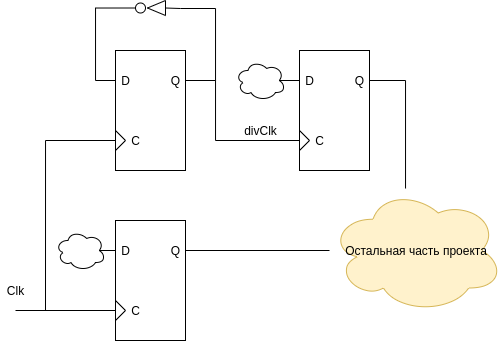
\includegraphics[width=0.5\linewidth]{course-scheme/images/clock-domain}
	\caption{Схема с одним доменом синхрочастоты}
	\label{fig:clock-domain}
\end{figure}


На Рисунке \ref{fig:multiclock-domain} показано несколько синхрочастот от различных источников. Ту часть проекта, которая управляется этими синхрочастотами, называют доменами синхрочастоты, и сигналы, осуществляющие передачу импульсов между этими асинхронными доменами синхрочастоты, называют путями пересечения домена синхрочастоты. Сигнал DA считают асинхронным сигналом в домене синхрочастоты, так как между генератором синхронизации A (clkA) и генератором синхронизации B (ClkB) не существуют постоянные соотношения фазы и времени. 




\begin{figure}[h!]
	\centering
	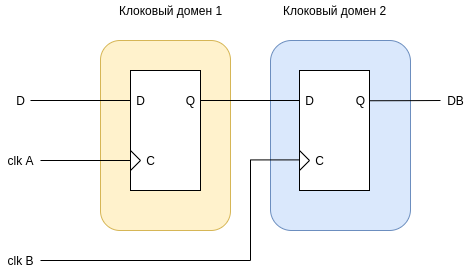
\includegraphics[width=0.7\linewidth]{course-scheme/images/multiclock-domain}
	\caption{Путь домена синхрочастоты}
	\label{fig:multiclock-domain}
\end{figure}


\section{Основные принципы}

При разработке ультисинхрочастотных проектов следует уделять особое внимание стабильности сигнала. Когда сигнал пересекает домен синхрочастоты, то он появляется в новом домене синхрочастоты как асинхронный сигнал и должен быть засинхронизирован.

Синхронизация предотвращает в новом домене синхрочастоты метастабильное состояние первого запоминающего элемента схемы (триггера), и это позволяет в новом домене работать уже со стабильным сигналом.

\textit{Метастабильность} --- это неспособность триггера достигнуть известного состояния в определенный момент времени. Когда триггер входит в метастабильное состояние, то невозможно предсказать ни уровень выходного напряжения элемента, ни период времени, за который этот выход перейдет к правильному уровню напряжения. 

В течение этого переходного времени выход триггера будет находиться на некотором промежуточном уровне напряжения или колебаться и может передать этот недопустимый уровень сигнала со своего выхода к другим триггерам схемы.

\section{Решение проблемы метастабильности}

С целью решения проблемы метастабильности применяются каскады стабилизирующих триггеров, включенных последовательно. Рассмотрим это решение.


Простейший синхронизатор представляет собой два триггера, включенных последовательно без какой-либо комбинационной схемы между ними. Такая схема проекта гарантирует, что первый триггер выходит из своего метастабильного состояния, и его выход переходит в устойчивое состояние перед тем, как второй триггер сохраняет его. Необходимо также разместить эти триггеры, насколько возможно, ближе друг к другу для того, чтобы гарантировать наименьшую расфазировку тактовых сигналов между ними. 

Другой тип ячейки синхронизатора представляет собой два близко расположенных триггера без какой-либо комбинационной логики между ними. Для того чтобы синхронизация работала должным образом, сигнал, пересекающий домен синхрочастоты, должен проследовать от триггера в домене синхрочастоты источника сигнала к первому триггеру синхронизатора, не пройдя через комбинационную логику.

Синхронизацию в домене называют привязкой входного сигнала к тактовой частоте
домена, т. е. все изменения этого сигнала в домене будут происходить по фронту или срезу
тактового сигнала домена, а не родительского тактового сигнала. На Рисунке \ref{fig:sync-triggers}) приведена схема традиционного синхронизатора из
двух триггеров (сдвиговый регистр) для одиночного сигнала. Схема синхронизации приведена на Рисунке \ref {fig:sync-scheme}.

\begin{figure}[h!]
	\centering
	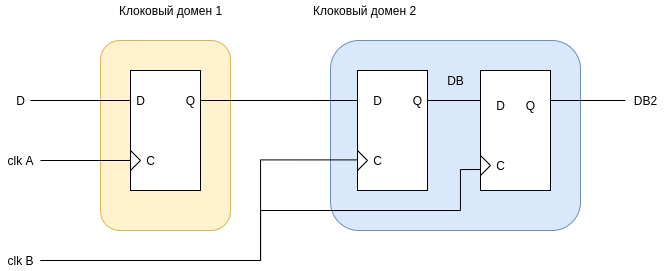
\includegraphics[width=0.6\linewidth]{course-scheme/images/sync-triggers}
	\caption{Триггеры синхронизации}
	\label{fig:sync-triggers}
\end{figure}

\begin{figure}[h!]
	\centering
	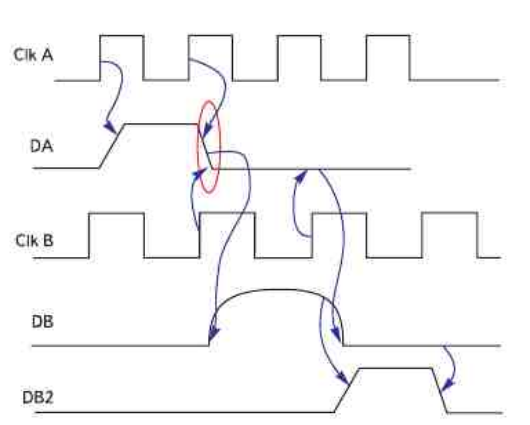
\includegraphics[width=0.3\linewidth]{course-scheme/images/sync-scheme}
	\caption{Схема синхронизации сигнала}
	\label{fig:sync-scheme}
\end{figure}
%\clearpage
%\vspace{2ex}

Данный способ борьбы с метастабильностью будет в дальнейшем использован при разработке узла ресихронизации данных.

\section{Асинхронная очередь}

Во многих проектах необходимо передавать из одного домена в другой не только несколько одиночных сигналов, но и сигналы типа шин: шины данных, адреса и шины управления.

В этих задачах активно используются буферы типа FIFO и специальные протоколы для процедуры установления связи. Особенно полезной оказывается асинхронная очередь, позволяющая производить запись и чтение по синхросигналам двух клоковых доменов.
Данная схема позволяет быстро и удобно передавать данные в реальном времени между двумя разными областями синхронизации.

На Рисунке \ref{fig:async-fifo} приведена схема использования двухпорторой оперативной памяти, позволяющей осуществлять передачу данных между частями устройства, использующими синхросигналы разной частоты.

\begin{figure}[h!]
	\centering
	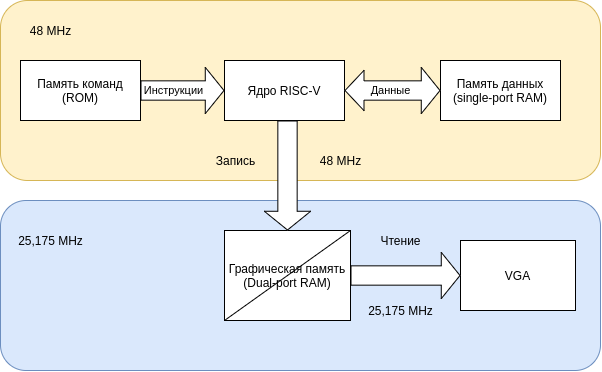
\includegraphics[width=0.65\linewidth]{course-scheme/images/dual-port-ram}
	\caption{Двухпортовая оперативная память}
	\label{fig:async-fifo}
\end{figure}

Двухпортовая память с независимыми тактовыми сигналами --- аппаратный блок, используемый в современных FPGA и в технологических библиотеках для заказных микросхем. Чтение и запись производится совершенно независимо через два отдельных порта.

Единственным ограничением является одновременное обращение на запись и чтение по одному и тому же адресу памяти --- оно может привести к неопределенному результату. На основе такого блока памяти зачастую создается модуль FIFO, который позволяет с одной стороны записывать данные из одного тактового домена, а с другой — забирать в другой тактовый домен. Заодно логика FIFO следит за тем, чтобы не происходило обращения к одной и той же ячейке памяти.

Данный узел работает по следующему принципу. 
\begin{enumerate}
	\item Источник данных загружает данные в асинхронную очередь. Тактирование производится по тактовому сигналу источника данных.
	\item Потребитель данных считывает данные из асинхронной очереди в исходном порядке. Тактирование производится по тактовому сигналу потребителя данных. 
\end{enumerate}




\clearpage
\chapter{ПРОЕКТИРОВАНИЕ ЦИФРОВОГО УСТРОЙСТВА}

\label{sec:design}
В данном разделе освещается разработка функциональной и структурной схем устройства по ресинхронизации данных. Определим структурные элементы устройства, принцип и порядок его работы.

\section{Организация взаимодействия с устройством}
Взаимодействие с устройством производится посредством передачи восьмибитного слова на вход wdata. Аппаратный блок осуществляет запись данных во внутреннюю память по сигналам тактового генератора домена источника данных wclk, основываясь на состоянии входных сигналов wrst, wen и служебных сигналов wr\_full,  wptr, rptr.

Чтение из устройства ресинхронизации производится посредством считывания тридцатидвухразрядного слова, составляемого из четырех последовательно поданных на вход восьмиразрядных слов в порядке \textit{от старшего к младшему} (англ. big-endian), генерируемого на выходе rdata. Аппаратный блок осуществляет чтение данных из внутренней памяти по сигналам тактового генератора домена получателя данных, основываясь на состоянии входных сигналов rrst, ren  r\_empty wptr, rptr, rdredy.

\section{Организация памяти}

Устройство хранит данные в собственной памяти. Устройство может одновременно хранить шестнадцать восьмибитных слов, используя для их адресации пятиразрядный адрес, в котором старший бит призван реализовать возможность контроля заполнения и опустошения очереди. 

Возможность асинхронного сброса памяти не реализована в силу того, что обычно память в устройствах, реализуемых на ПЛИС представлена в виде блочной оперативной памяти и выделенной оперативной памяти. Эти ресурсы обычно не поддерживают сброс. Сброс возможно реализовать в регистрах. 



\section{Тактирование}
Управление устройством производится по двух синхросигналам wclk и rclk. С целью оптимальной работы цифрового устройства при передаче данных из одного домена синхросигнала в другой тактовые сигналы входного и выходного каналов сделаны независимыми, однако тактовая частота для выхода очереди составляет как минимум $\dfrac14$ от тактовой частоты входного интерфейса FIFO.

Для корректной передачи и предотвращения потери данных, а также с целью борьбы с метастабильностью в случае независимых тактовых сигналов используются группа синхронизирующих триггеров, которые передают текущее состояние адреса чтения и адреса записи между клоковыми доменами. Основываясь на значениях данных адресов делается вывод о заполненности и пустоте очереди. 

\section{Адресация}

Адресация в памяти реализована с помощью двух пятиразрядных переменных, хранящих адрес ячеек,  с которыми будут произведены операции чтения и записи при следующем синхросигнале.

Важной частью работы устройства является работа с памятью. Необходимо избежать потери и перезаписи не переданных данных. С этой целью на каждом шаге работы схемы осуществляется проверка и сравнивание адресов чтения и записи.

Во время работы схема хранит адреса в виде рефлексивного двоичного кода Грея. Выбор в сторону кода Грея сделан для снижения критичности ошибки определения адреса чтения или записи при его передаче. 

В случае использования кода Грея при переходе к следующему адресу изменяется только один бит, и даже если схема не сможет верно определить значение адреса~---~посчитает, что адреса не изменился, это не приведет к нарушению работы системы. 

В то время как при использовании прямого двоичного кода ошибка синхронизации неизбежна. При переходе могут изменяться все биты адреса (например при переходе $01111 \to 1000$). В данном случае значение адреса является полностью неопределенным. Это может привести к нарушению в работе устройства в целом.

Когда указатели чтения и записи равны, это указывает на то, что FIFO пуст. Эта ситуация возникает во время операции сброса или когда было произведено чтение последнего слова в FIFO, как показано на Рисунке \ref{fig:empty-fifo}.

\begin{figure}[h!]
	\centering
	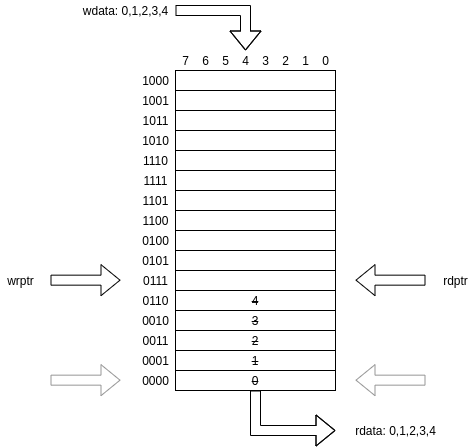
\includegraphics[width=0.7\linewidth]{course-scheme/images/empty-fifo}
	\caption{Все данные прочитаны. Очередь пуста}
	\label{fig:empty-fifo}
\end{figure}

Когда указатели чтения и записи снова равны, это означает, что очередь заполнена и дальнейшая запись не может быть произведена. Эта ситуация возникает, когда переменная адреса записи переполняется, как показано на Рисунке \ref{fig:full-fifo}.

\begin{figure}[h!]
	\centering
	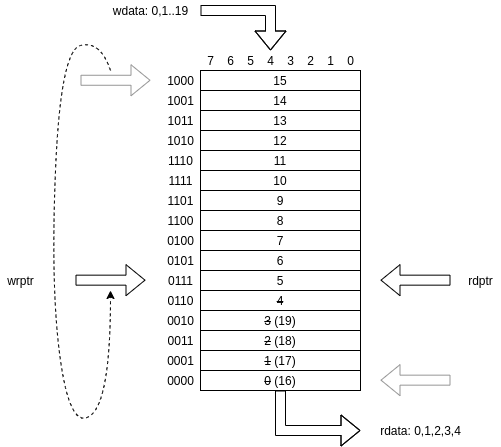
\includegraphics[width=0.7\linewidth]{course-scheme/images/full-fifo}
	\caption{Очередь заполнена. Запись не допустима}
	\label{fig:full-fifo}
\end{figure}

В обоих случаях адреса записи и чтения указывают на одну и ту же ячейку памяти, но при этом ситуации являются противоположными, что усложняет логику определения текущего состояния памяти цифрового устройства.

С целью определения текущего состояния асинхронной очереди необходимо использовать на один бит больше, чем требуется для адресации всех ячеек запоминающего устройства. Сравнение этого бита даст ответ о состоянии памяти в случае, когда указатели чтения и записи окажутся равны.

Пятиразрядные сигналы wr\_full и rd\_empty, позволяющие организовать корректную работу с устройством, формируются с помощью следующих логических условий.
\begin{align}
	 wr\_full = &\left(wptr  == \left\{!rptr[4:3],rptr[aw-2:0]\right\}\right);\\
	 &rd\_empty = \left(wptr  == rptr\right)
\end{align}

В устройстве необходимо реализовать проверку обращения к одному элементу памяти. Чтение по данному адресу должно быть заблокировано до тех пор, пока адрес записи не перестанет указывать на данную ячейку памяти.

При каждом приходящем тактовом сигнале устройство осуществляет сравнение адресов чтения и записи, предварительно производя с ними промежуточные действия. Приведем список преобразований и производимых операций.

\begin{itemize}
	\item перевод из прямого двоичного кода в рефлексивный код Грея;
	\item сохранение текущего значения в регистре;
	\item передача значения адреса в синхронизационные регистры;
	\item перевод из рефлексивного кода Грея в прямой двоичный код;
	\item синхронизация приходящего адреса генератором соседнего домена синхронизации;
	\item сравнение адресов чтения и записи.
\end{itemize}

Данные операции производятся с адресом чтения и записи отдельно. Порядок следования этих операций можно пронаблюдать на Рисунке \ref{fig:signal-process}.

\begin{figure}
	\centering
	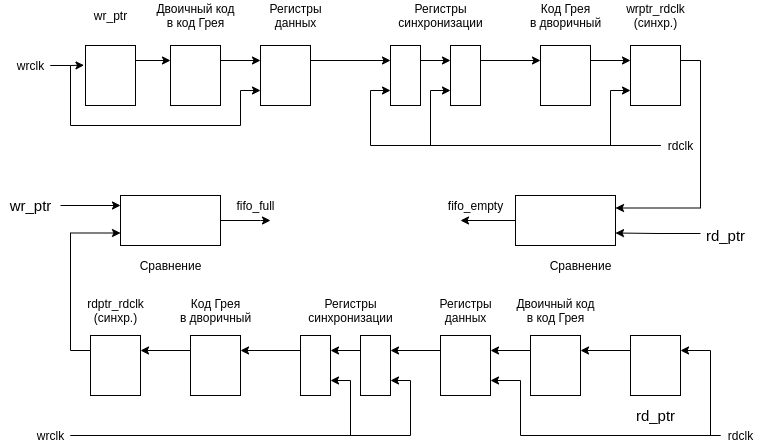
\includegraphics[width=1\linewidth]{course-scheme/images/signal-process}
	\caption{Обработка адресов чтения и записи}
	\label{fig:signal-process}
\end{figure}



\section{Функциональная схема}
Предлагается для построения устройства ресинхронизации данных, работающего в режиме очереди с независимыми тактовыми сигналами, использовать данную функциональную схему (см. Рисунок \ref{fig:unit-design}).

\begin{figure}[h!]
	\centering
	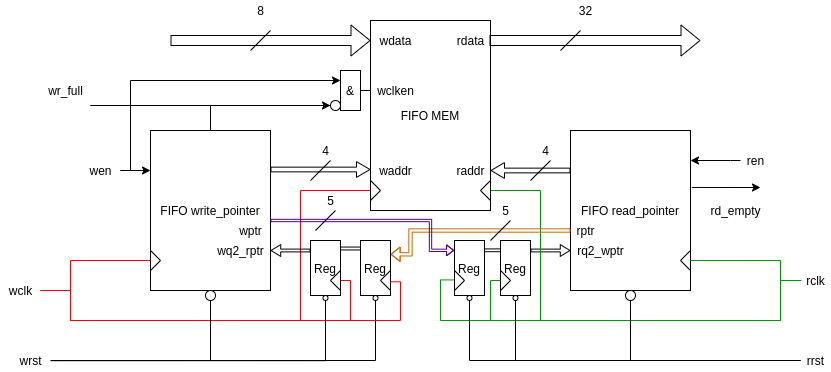
\includegraphics[width=1\linewidth]{course-scheme/images/unit-design}
	\caption{Функциональная схема устройства}
	\label{fig:unit-design}
\end{figure}


Приведем описание входов, выходов и служебных сигналов устройства (см. Таблицу \ref{tab:sig-ports}).

Также укажем используемые глобальные и локальные параметры, используемые при реализации устройства на языке описания аппаратуры Verilog (см. Таблицу \ref{tab:params}). С помощью данных параметров возможно произвести масштабирование устройства --- увеличить разрядность ячейки запоминающего устройства и их количество.

\begin{table}[htbp]
	\centering
	\fontsize{12}{16pt}\selectfont
	\caption{Параметры}
	\begin{tabular}{|l|p{0.5\linewidth}|c|}
		\hline
		\multicolumn{1}{|c}{\textbf{Название}} & \multicolumn{1}{|c|}{\textbf{Назначение}} & \multicolumn{1}{c|}{\textbf{Значение}} \\ \hline
		asize  &  разрядность адреса данных & 4 \\ \hline
		dsize  &  разрядность данных в битах & 8 \\ \hline
	\end{tabular}
	\label{tab:params}
\end{table}

Аппаратный блок по ресинхронизации данных разрабатывается для использования в совокупности с более сложными элементами и выполняет роль служебного блока хранения и передачи данных.

И



\begin{table}[h!]
	\fontsize{12}{16pt}\selectfont
	\centering
	\caption{Сигналы входы и выходы устройства}
	\label{tab:sig-ports}
	\begin{tabular}{|l|l|c|}
		\hline
		\multicolumn{1}{|c}{\textbf{Название}} & \multicolumn{1}{|c|}{\textbf{Назначение}} & \multicolumn{1}{c|}{\textbf{Разрядность}} \\ \hline
		mem  &  ячейки памяти очереди & [8:0] [0:15] \\ \hline
		rbin  &  текущий адрес чтения в бинарном коде & [4:0] \\ \hline
		rbinnext  &  адрес чтения в бинарном коде в следующем такте & [4:0] \\ \hline
		rclk  &  тактирование на чтение данных & 1 \\ \hline
		rdata  &  данные на чтение & [31:0] \\ \hline
		rden  &  разрешение на чтение & 1 \\ \hline
		rdredy  &  готовность выдать данные & 1 \\ \hline
		rempty  &  сигнал пустоты очереди (прочтено все, что записано) & 1 \\ \hline
		rempty\_next  &  пустота очереди на следующем такте & 1 \\ \hline
		rgray  &  текущий адрес чтения в коде Грея & [4:0] \\ \hline
		rgraynext  &  адрес чтения в коде Грея в следующем такте & [4:0] \\ \hline
		rq1\_wgray  &  адрес чтения в первом синхро-триггере & [4:0] \\ \hline
		rq2\_wgray  &  адрес чтения во втором синхро-триггере & [4:0] \\ \hline
		rrstn  &  сброс указателя чтения & 1 \\ \hline
		wbin  &  текущий адрес записи в бинарном коде & 1 \\ \hline
		wbinnext  &  адрес записи в бинарном коде в следующем такте & [4:0] \\ \hline
		wclk  &  Тактирование на запись данных & 1 \\ \hline
		wdata  &  данные на запись & [7:0] \\ \hline
		wfull  &  сигнал заполнения очереди & 1 \\ \hline
		wfull\_next  &  заполненность очереди на следующем такте & 1 \\ \hline
		wgray  &  текущий адрес записи в коде Грея & [4:0] \\ \hline
		wgraynext  &  адрес записи в коде Грея в следующем такте & [4:0] \\ \hline
		wq1\_rgray  &  адрес записи в первом синхро-триггере & [4:0] \\ \hline
		wq2\_rgray  &  адрес записи во втором синхро-триггере & [4:0] \\ \hline
		wren  &  разрешение на запись & 1 \\ \hline
		wrstn  &  сброc указателя записи & 1 \\ \hline
	\end{tabular}
\end{table}
\normalsize
\clearpage







\clearpage
\clearpage

%\cite{d2004mysql},\cite{baldinLatex}, \cite{converse2004php5}, \cite{yurt2011dev}.

\backmatter %% Здесь заканчивается нумерованная часть документа и начинаются ссылки и
            %% заключение

\Conclusion % заключение к отчёту

Результатом работы над данной курсовой работой является ознакомление с проблематикой разработки мультисинхронных устройств, реализация цифрового устройства ресинхронизации данных, представляющего собой асинхронную очередь данных, тактируемого двумя независимыми синхросигналами.

В ходе данной работы были проведены мероприятия по разработке функциональной и структурной схемы цифрового устройства и устройств, необходимых для его работы; созданию модуля, реализующего устройство ресинхронизации данных на языке описания аппаратуры Verilog; включению данного устройства в состав сложных устройств и проведение его отладки и тестирования.

Цели и задачи по реализации устройства для ресинхронизации данных выполнены. 

%%% Local Variables: 
%%% mode: latex
%%% TeX-master: "rpz"
%%% End: 


% % Список литературы при помощи BibTeX
% Юзать так:
%
% pdflatex rpz
% bibtex rpz
% pdflatex rpz

\bibliographystyle{gost780u}
\bibliography{course-scheme/rpz}

%%% Local Variables: 
%%% mode: latex
%%% TeX-master: "rpz"
%%% End: 


\cite{goncharovskyMaj}. \cite{ushenina}.\cite{hata2012fpga}, \cite{cummings2002simulation},\cite{tarasov2011}, \cite{stempcovsky}.

\appendix   % Тут идут приложения
%
%\chapter{Картинки}
\label{cha:appendix1}

\begin{figure}
\centering
\caption{Картинка в приложении. Страшная и ужасная.}
\end{figure}

%%% Local Variables: 
%%% mode: latex
%%% TeX-master: "rpz"
%%% End: 

%\chapter{Еще картинки}
\label{cha:appendix2}

\begin{figure}
\centering
\caption{Еще одна картинка, ничем не лучше предыдущей. Но надо же как-то заполнить место.}
\end{figure}

%%% Local Variables: 
%%% mode: latex
%%% TeX-master: "rpz"
%%% End: 





\begin{table}
	\begin{tabular}{l|l}
		\hline
	\end{tabular}
\end{table}




\end{document}

%%% Local Variables:
%%% mode: latex
%%% TeX-master: t
%%% End:
